\chapter{User Documentation} % User guide
\label{ch:user}

This chapter contains a brief description of the project, a guide on how
to install and run the analyzer, and the way to use.

\section{Project Description} % Enumerations and lists
This project is a log analyzer working alongside the PipeRT framework
with its profiler. The project aims to analyze the continuous stream of
data coming from the PipeRT's profiler, in a server-client relationship.

The analyzer was build using python in the backends and Javascript in the frontend,
it provides various checkers to investigate the sanity of the pipeline created by
user using PipeRT, graphs associated with the measurements prepared by the checkers, and visualization
of the pipeline and how the channels are structured.

The analyzer in itself was built to be an analyzing framework where
extensibility was the key and will be in the design decisions, so as a result,
it is relatively easy to add new features and already prepared to be extended
by new checkers and measurements.


\section{Installation Guide}
PipeRT is currently supporting Linux only, but soon,
it will support Windows as well. That said, the steps to install
the analyzer are the same in both operations systems.

The \textbf{\url{log_analyzer}} folder inside the PipeRT project folder
is where all of the Installation steps will take place.

Python 3.9 should be installed on the operating system. All the
requirements can be installed by typing the following command in
the terminal or the command prompt.

\begin{lstlisting}[language=bash, caption={Install requirements},captionpos=b]
	$ pip install requirements.txt
\end{lstlisting}

It is also recommended to create a python virtual environment
before installing the requirements, in order to have a separate
environment for the analyzer. The commands to create and run the environment
are:

\begin{lstlisting}[language=bash, caption={Create virtual environment},captionpos=b]
	$ python3 -m venv venv	
	$ source venv/bin/activate
\end{lstlisting}


\subsection{Running} % Framing figures
In order to run the analyzer make sure to be inside the
\textbf{\url{log_analyzer}} folder and type the following
command:

\begin{lstlisting}[language=bash, caption={Start application},captionpos=b]
	$ python start.py
\end{lstlisting}

This will start the application, so once you type \url{127.0.0.1:5000}
in the browser (Firefox recommended). You will be able to see the following:

\begin{figure}[H]
	\centering
	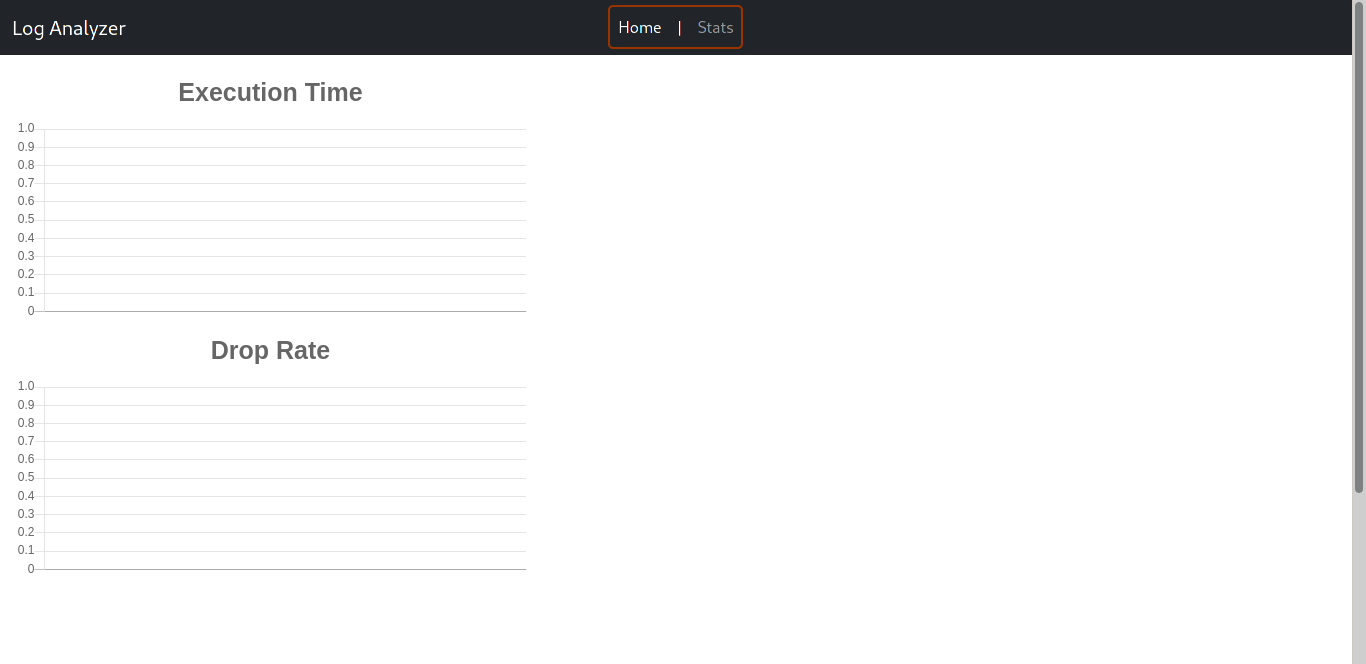
\includegraphics[width=0.9\textwidth,height=175px]{images/start.png}
	\caption{Start of the application}
	\label{fig:empty_page}
\end{figure}

\section{Client-Server Configuration} % Tables
To establish a connection between the profiler (Client)
and the log analyzer (server), there should be modifications in both
sides.

\subsection{Server Side}

The profiler is the utility for monitoring the DSP pipeline and sending logs,
it has 3 arguments, first is \textbf{\url{destination_uri}},
which describes the destination and the used protocol, udp and file
are the protocol options in the profiler currently. The Second argument
is \textbf{\url{aggregation_time_msec}} which is the time in milliseconds to wait 
before gathering monitoring data again, so it determines how often aggregated
log data is sent to the log processor, if not given that means not to collect
periodically. The third argument is \textbf{\url{buffer_size}}, it controls the size
of buffer which is filled to be sent at once, the default value depends on the
protocol chosen.

To establish a connection with the analyzer, the udp protocol
is the one to choose, the IP and socket are based on the user
preference.

Adding the profiler to the scheduler is the last step to configure
the server-side, and the following example showing how to add the profiler.

\begin{lstlisting}[language=c++, caption={Adding profiler},captionpos=b]
	pipert::Scheduler sch(0, pipert::Profiler("udp:127.0.0.1:8000"));
\end{lstlisting}

\subsection{Client Side}\label{client_side}
On the client-side, the same port number that has been provided to the profiler
should be added in the \textbf{config.json} inside the \textbf{\url{log_analyzer}} folder. same for
the IP as well.

\begin{lstlisting}[language=bash, caption={connection configuration},captionpos=b]
{
	"PORT": "8000"
	"IP": "127.0.0.1"
}
\end{lstlisting}

An important note: The log analyzer will start analyzing and
draw the visualization, at the end of the first packet cycle \ref{g_config}, so, 
the web page will be the same as \ref{fig:empty_page} 
until the completion of the cycle.

\section{Analyzer Configuration}
The log analyzer is made to check the sanity and analyze various
applications and systems, so having a configuration, was essential.

The configuration is a JSON (JavaScript Object Notation) file,
the choice of the format to be JSON was due to its
lightweight, well-known among developers, and simplicity. 
The config.json configuration file consists of 2 main parts, 
general and checkers' configurations. Let's enumerate these configurations.

\begin{lstlisting}[language=bash, caption={Sample configuration},captionpos=b, label={lst:sample_confing}]
	{
		"PORT": "8000",
		"IP": "127.0.0.1",
		"PACKET_CYCLE_THRESHOLD": 1000,
		"checkers": [
			{
				"name": "frozen_checker",
				"enabled": true,
				"parameters": {
					"FROZEN_LIMITS": 20
				}
			}
		]
	}
\end{lstlisting}

\subsection{General Configuration} \label{g_config}
Consist of 3 configurations, \textbf{PORT}, \textbf{IP}, 
and \textbf{\url{PACKET_CYCLE_THRESHOLD}}. The first two were discussed in \ref{client_side}.

The \textbf{\url{PACKET_CYCLE_THRESHOLD}} is an integer value that describes
how many packets should the analyzer receive before running the checkers once
and these packets' events will be stored in the channels and when the cycle
finishes (when the number of packets received is equal to \textbf{\url{PACKET_CYCLE_THRESHOLD}}), these
events will be deleted from the channels and a new packets cycle starts.

\begin{figure}[H]
	\centering
	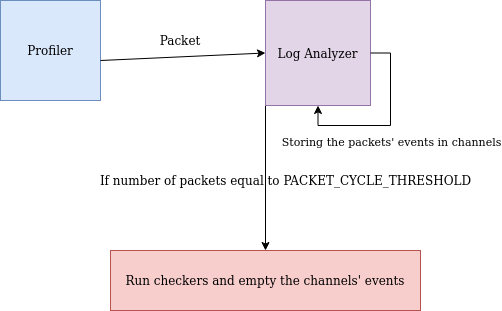
\includegraphics[width=0.9\textwidth,height=200px]{images/packets_cycle.png}
	\caption{Packets cycle}
	\label{fig:packets_cycle}
\end{figure}

\subsection{Checkers' Configuration}
As it is shown from \ref{lst:sample_confing}, the checkers' configuration is a
list of dictionaries where each dictionary is a checker's configuration. Each configuration
contains the checker's name in the \textbf{name} field, whether it should work or not in
the \textbf{enabled} field, and a \textbf{parameters} field where the parameter
of the checker can be created or changed.

The \textbf{name} field should be the same name as the file of the checker 
without the extension (.py). And that is how the dynamic importing module in 
the project will be able to import the checker with its configuration \ref{}.

The \textbf{enabled} field is a boolean field to turn on or off the checker.

The \textbf{parameters} field is a dictionary with as many keys as the checker's
parameters. These values can be changed based on the DSP application using the
analyzer, and it is the user's responsibility to assign the appropriate values.

In the next section, we will discuss the implemented checkers in detail.
\begin{table}[H]
	\centering
	\begin{tabular}{ | m{0.25\textwidth} | m{0.65\textwidth} | }
		\hline
		\textbf{Phasellus tortor} & \textbf{Aenean consequat} \\
		\hline \hline
		\emph{Sed malesuada} & Aliquam aliquam velit in convallis ultrices. \\
		\hline
		\emph{Purus sagittis} &  Quisque lobortis eros vitae urna lacinia euismod. \\
		\hline
		\emph{Pellentesque} & Curabitur ac lacus pellentesque, eleifend sem ut, placerat enim. Ut auctor tempor odio ut dapibus. \\
		\hline
	\end{tabular}
	\caption{Maecenas tincidunt non justo quis accumsan}
	\label{tab:example-1}
\end{table}

\subsection{Sorok és oszlopok egyesítése} % Multi rows and multi columns

Mauris a dapibus lectus. Vestibulum commodo nibh ante, ut maximus magna eleifend vel. Integer vehicula elit non lacus lacinia, vitae porttitor dolor ultrices. Vivamus gravida faucibus efficitur. Ut non erat quis arcu vehicula lacinia. Nulla felis mauris, laoreet sed malesuada in, euismod et lacus. Aenean at finibus ipsum. Pellentesque dignissim elit sit amet lacus congue vulputate.

\begin{table}[htb]
	\centering
	\begin{tabular}{ | c | r | r | r | r | r | r | }
		\hline
		\multirow{2}{*}{\textbf{Quisque}} & \multicolumn{2}{ c | }{\textbf{Suspendisse}} & \multicolumn{2}{ c | }{\textbf{Aliquam}} & \multicolumn{2}{ c | }{\textbf{Vivamus}} \\
		\cline{2-7}
		& Proin & Nunc & Proin & Nunc & Proin & Nunc \\
		\hline \hline		
		Leo & 2,80 MB & 100\% & 232 KB & 8,09\% & 248 KB & 8,64\% \\
		\hline
		Vel & 9,60 MB & 100\% & 564 KB & 5,74\% & 292 KB & 2,97\% \\
		\hline
		Auge & 78,2 MB & 100\% & 52,3 MB & 66,88\% & 3,22 MB & 4,12\% \\
		\hline 
	\end{tabular}
	\caption[Rövid cím a táblázatjegyzékbe]{Vivamus ac arcu fringilla, fermentum neque sed, interdum erat. Mauris bibendum mauris vitae enim mollis, et eleifend turpis aliquet.}
	\label{tab:example-2}
\end{table}

\subsection{Több oldalra átnyúló táblázatok} % Long tables over multiple pages

Nunc porta placerat leo, sit amet porttitor dui porta molestie. Aliquam at fermentum mi. Maecenas vitae lorem at leo tincidunt volutpat at nec tortor. Vivamus semper lacus eu diam laoreet congue. Vivamus in ipsum risus. Nulla ullamcorper finibus mauris non aliquet. Vivamus elementum rhoncus ex ut porttitor.

\begin{center}
	\begin{longtable}{ | p{0.3\textwidth} | p{0.7\textwidth} | }
		
		\hline
		\multicolumn{2}{|c|}{\textbf{Praesent aliquam mauris enim}}
		\\ \hline
		
		\emph{Suspendisse potenti} & \emph{Lorem ipsum dolor sit amet}
		\\ \hline \hline
		\endfirsthead % első oldal fejléce
		
		\hline
		\emph{Suspendisse potenti} & \emph{Lorem ipsum dolor sit amet}
		\\ \hline \hline
		\endhead % többi oldal fejléce
		
		\hline
		\endfoot % többi oldal lábléce
		
		\endlastfoot % utolsó oldal lábléce
		
		\emph{Praesent}
		& Nulla ultrices et libero sit amet fringilla. Nunc scelerisque ante tempus sapien placerat convallis.
		\\ \hline
		
		\emph{Luctus}
		& Integer hendrerit erat massa, non hendrerit risus convallis at. Curabitur ultrices, justo in imperdiet condimentum, neque tortor luctus enim, luctus posuere massa erat vitae nibh.
		\\ \hline
		
		\emph{Egestas}
		& Duis fermentum feugiat augue in blandit. Mauris a tempor felis. Pellentesque ultricies tristique dignissim. Pellentesque aliquam semper tristique. Nam nec egestas dolor. Vestibulum id elit quis enim fringilla tempor eu a mauris. Aliquam vitae lacus tellus. Phasellus mauris lectus, aliquam id leo eget, auctor dapibus magna. Fusce lacinia felis ac elit luctus luctus.
		\\ \hline
		
		\emph{Dignissim}
		& Praesent aliquam mauris enim, vestibulum posuere massa facilisis in. Suspendisse potenti. Nam quam purus, rutrum eu augue ut, varius vehicula tellus. Fusce dui diam, aliquet sit amet eros at, sollicitudin facilisis quam. Phasellus tempor metus vel augue gravida pretium. Proin aliquam aliquam blandit. Nulla id tempus mi. Fusce in aliquam tortor.
		\\ \hline
		
		\emph{Pellentesque}
		& Donec felis nibh, imperdiet a arcu non, vehicula gravida nibh. Quisque interdum sapien eu massa commodo, ac elementum felis faucibus.
		\\ \hline
		
		\emph{Molestie}
		& Cras ullamcorper tellus et auctor ultricies. Maecenas tincidunt euismod lectus nec venenatis. Suspendisse potenti. Pellentesque pretium nunc ut euismod cursus. Nam venenatis condimentum quam. Curabitur suscipit efficitur aliquet. Interdum et malesuada fames ac ante ipsum primis in faucibus.
		\\ \hline
		
		\emph{Vivamus semper}
		& In purus purus, faucibus eu libero vulputate, tristique sodales nunc. Nulla ut gravida dolor. Fusce vel pellentesque mi, vel efficitur eros. Nunc vitae elit tellus. Sed vestibulum auctor consequat. 
		\\ \hline
		
		\emph{Condimentum}
		& Nulla scelerisque, leo et facilisis pretium, risus enim cursus turpis, eu suscipit ipsum ipsum in mauris. Praesent eget pulvinar ipsum, suscipit interdum nunc. Nam varius massa ut justo ullamcorper sollicitudin. Vivamus facilisis suscipit neque, eu fermentum risus. Ut at mi mauris.
		\\ \hline
		
		\caption{Praesent ullamcorper consequat tellus ut eleifend}
		\label{tab:example-3}		
	\end{longtable}
\end{center}